\documentclass[12pt,a4paper,notitlepage]{article}

\usepackage{./styles/year-2000}

\addbibresource{year-2000.bib}

%\syntaxonly

\newcommand*{\foottitle}{Year 2000 Problem}

\title{
	
\includegraphics[scale=0.15]{feuplogo.jpg}\\
	{\Huge Year 2000 Problem}\\
	{\Large Software failures}\\
	{\normalsize Software Engineering 2018}
}

\author{
	Diogo Yaguas\\ \text{up201606165}
}

\begin{document}
\maketitle
\thispagestyle{empty}

\section{Synopsys}

Also known as the millennium bug, it was a problem in the coding of computerized systems that was projected to create havoc in computers and computer networks around the world at the beginning of the year 2000. After more than a year of international alarm, feverish preparations, and programming corrections, few significant failures occurred in the transition from December 31, 1999, to January 1, 2000.

Computer programmers have been in the habit of using two-digit placeholders for the year portion of the date in their software. For example, the expiration date for a typical insurance policy or credit card was stored in a computer file in MM/DD/YY format.

\begin{wrapfigure}[10]{l}[1em]{0.40\textwidth}
	\vspace{-0.5\baselineskip}
	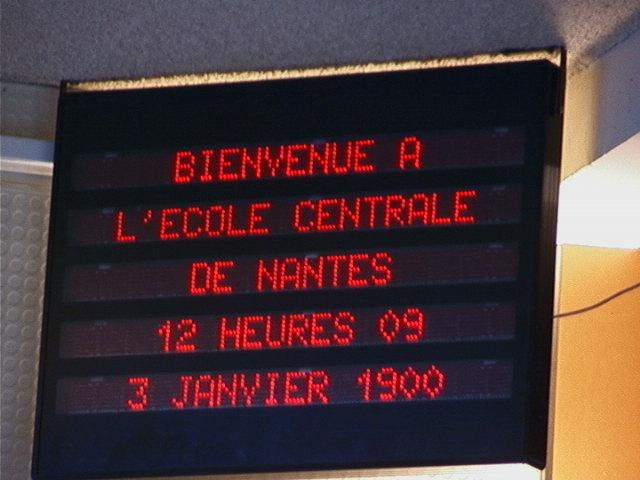
\includegraphics[scale=0.265]{french-bug.jpg}
\end{wrapfigure}

The 2-digit year format created a problem for most programs when "00" was entered for the year. The software does not know whether to interpret "00" as "1900" or "2000". Most programs, therefore, default to 1900. That is, the code that most programmers wrote either prepends "19" to the front of the two-digit date, or it makes no assumption about the century and therefore, by default, it is "19". This wouldn't be a problem except that programs perform lots of calculations on dates. For example, to calculate how old you are a program will take today's date and subtract your birthdate from it. That subtraction works fine on two-digit year dates until today's date and your birthdate are in different centuries. Then the calculation no longer works. For example, if the program thinks that today's date is 1/1/00 and your birthday is 1/1/65, then it may calculate that you are -65 years old rather than 35 years old. As a result, date calculations give erroneous output and software crashes or produces the wrong results.

The Y2K problem was not limited to computers running conventional software, however. Many devices containing computer chips, ranging from elevators to temperature-control systems in commercial buildings to medical equipment, were believed to be at risk, which necessitated the checking of these “embedded systems” for sensitivity to calendar dates.

\begin{wrapfigure}[9]{r}[1em]{0.55\textwidth}
	\vspace{-0.5\baselineskip}
	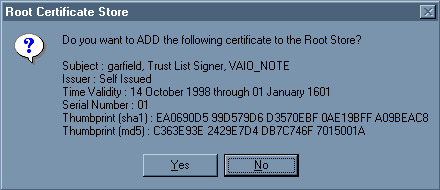
\includegraphics[scale=0.55]{root-certificate.jpg}
\end{wrapfigure}

An estimated 300 billion dollars was spent (almost half in the United States) to upgrade computers and application programs to be Y2K-compliant. As the first day of January 2000 dawned and it became apparent that computerized systems were intact, reports of relief filled the news media. These were followed by accusations that the likely incidence of failure had been greatly exaggerated from the beginning. Those who had worked in Y2K-compliance efforts insisted that the threat had been real. They maintained that the continued viability of computerized systems was proof that the collective effort had succeeded. In following years, some analysts pointed out that programming upgrades that had been part of the Y2K-compliance campaign had improved computer systems and that the benefits of these improvements would continue to be seen for some time to come.

Several very different approaches were used to solve the Year 2000 problem in legacy systems. Three of them follow:

\subsection{Date expansion}
Two-digit years were expanded to include the century (becoming four-digit years) in programs, files, and databases. This was considered the "purest" solution, resulting in unambiguous dates that are permanent and easy to maintain. However, this method was costly, requiring massive testing and conversion efforts, and usually affecting entire systems.

\subsection{Date re-partitioning}
In legacy databases whose size could not be economically changed, six-digit year/month/day codes were converted to three-digit years (with 1999 represented as 099 and 2001 represented as 101, etc.) and three-digit days (ordinal date in year). Only input and output instructions for the date fields had to be modified, but most other date operations and whole record operations required no change. This delays the eventual roll-over problem to the end of the year 2899.

\subsection{Windowing}
Two-digit years were retained, and programs determined the century value only when needed for particular functions, such as date comparisons and calculations. (The century "window" refers to the 100-year period to which a date belongs). This technique, which required installing small patches of code into programs, was more straightforward to test and implement than date expansion, thus much less costly. While not a permanent solution, windowing fixes were usually designed to work for several decades. This was thought acceptable, as older legacy systems tend to eventually get replaced by newer technology.

\subsection{Software Solutions}
In 1996, Rudy Rupak created the Millennium Bug Kit. This freeware solution was one of the first downloadable solutions on the internet at the time and was found in one in four computers and marketed through Planet City Software as Millennium Bug Compliance Kit.

\nocite{*}

\printbibliography

\end{document}